\documentclass{beamer}
\usepackage{float}
\usepackage{graphicx}
\usepackage{marginnote}
\usepackage{pgfgantt}
\usepackage{pdflscape}
\usepackage{wrapfig}
\usepackage{tikz}
\usetikzlibrary{matrix}
\usetikzlibrary{shapes,arrows}
\renewcommand{\footnoterule}{%
  \kern -3pt
  \hrule width \textwidth height 0.5pt
  \kern 2pt
}
\tikzstyle{decision} = [diamond, draw, fill=white!20, 
    text width=6em, text badly centered, node distance=3cm, inner sep=1pt]
\tikzstyle{block} = [rectangle, draw, fill=white!20, 
    text width=5em, text centered, rounded corners, minimum height=3em]
\tikzstyle{line} = [draw, -latex']
\tikzset{
  treenode/.style = {align=center, inner sep=0pt, text centered,
    font=\sffamily},
 arn_n/.style = {treenode, circle, white,  font=\sffamily, draw=black,
    fill=black, text width=1.5em}
}

\mode<presentation> {

\setbeamertemplate{footline}[page number] % To replace the footer line in all slides with a simple slide count uncomment this line

\setbeamertemplate{navigation symbols}{} % To remove the navigation symbols from the bottom of all slides uncomment this line
}

\usepackage{graphicx} % Allows including images
\usepackage{booktabs} % Allows the use of \toprule, \midrule and \bottomrule in tables

\title[Short title]{Random Number Generation using Genetic Programming: Design} % The short title appears at the bottom of every slide, the full title is only on the title page

\author{Philip Leonard} % Your name
\institute[UoL] % Your institution as it will appear on the bottom of every slide, may be shorthand to save space
{
University of Liverpool \\ % Your institution for the title page
\medskip
Primary Supervisor: Dr. David Jackson\\ Secondary Supervisor: Professor Paul E. Dunne\\
\medskip
\textit{sgpleona@student.liverpool.ac.uk} % Your email address
}
\date{} % Date, can be changed to a custom date

\begin{document}

\begin{frame}
\titlepage % Print the title page as the first slide
\end{frame}

\begin{frame}
\frametitle{Presentation Overview} % Table of contents slide, comment this block out to remove it
\tableofcontents % Throughout your presentation, if you choose to use \section{} and \subsection{} commands, these will automatically be printed on this slide as an overview of your presentation
\end{frame}

%----------------------------------------------------------------------------------------
%	PRESENTATION SLIDES
%----------------------------------------------------------------------------------------

%------------------------------------------------
\section{Project Overview} % Sections can be created in order to organize your presentation into discrete blocks, all sections and subsections are automatically printed in the table of contents as an overview of the talk
%------------------------------------------------

\begin{frame}
\frametitle{Project Overview}
The project can be broken down into 3 main stages, and therefore 3 design stages;\\~\\
\begin{itemize}
  \item[1.] Evolving a Random Number Generator (RNG) by means of \textbf{Genetic Programming} (GP) in C using Koza's paper \cite{kozarng}.\\~\\
  \item[2.] Evolving a Random Number Generator (RNG) by means of \textbf{Single Node Genetic Programming} (SNGP) in C using Jacksons paper \cite{jacksonsngp2}.\\~\\
  \item[3.] Compare and evaluate GP and SNGP methods for this application and then compare their evolved RNGs against other Pseudo and True Random Number Generators
\end{itemize}
\end{frame}

%GP APPROACH
%------------------------------------------------
\section{Design}
\subsection{Genetic Programming Design}
\begin{frame}
\frametitle{Genetic Programming Design}

\begin{columns}[T]
\begin{column}{0.75\textwidth}
\begin{itemize}
\item[-]The goal is to genetically breed a RNG to randomise a sequence of binary digits.\\~\\
\item[-]The input to the RNG is the sequence $J$, which runs from $i = 1$ to $2^{14}$. \\~\\
\item[-] The output is a sequence of random binary digits of size $J$. \\~\\
\item[-]The binary digit at location $i$ is determined by the LSB (Least Significant Bit) of the output from the RNG on the $i^{th}$ input. \\~\\
\end{itemize}
\end{column}
\begin{column}{0.35\textwidth}

\begin{figure}
\caption{GP flowchart}
\label{simpleflow}
\resizebox{3.5cm}{6cm}{
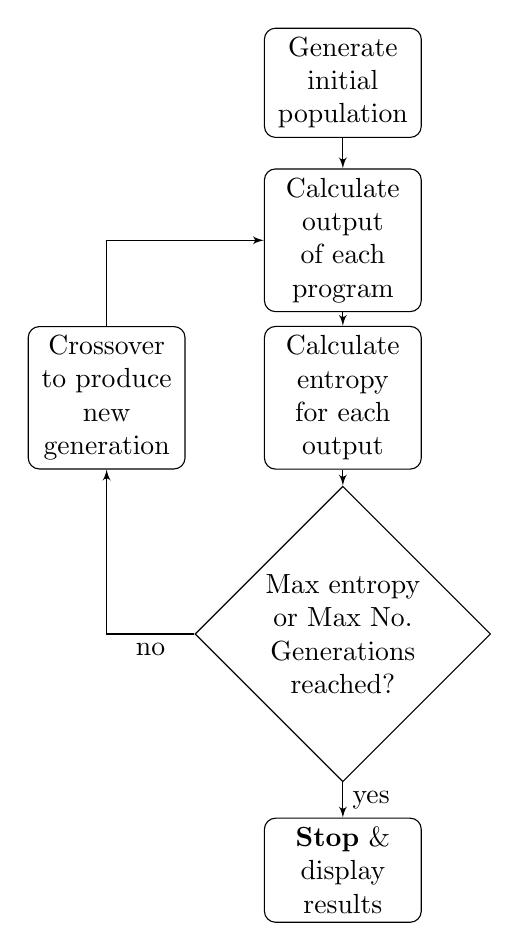
\begin{tikzpicture}[ node distance = 2cm, auto]
    % Place nodes
    \node [block] (init) {Generate initial population};
    \node [block, below of=init] (identify) {Calculate output of each program};
    \node [block, below of=identify] (evaluate) {Calculate entropy for each output};
    \node [block, left of=evaluate, node distance=3cm] (update) {Crossover to produce new generation};
    \node [decision, below of=evaluate] (decide) {Max entropy or Max No. Generations reached?};
    \node [block, below of=decide, node distance=3cm] (stop) {\textbf{Stop} \& display results};
    % Draw edges
    \path [line] (init) -- (identify);
    \path [line] (identify) -- (evaluate);
    \path [line] (evaluate) -- (decide);
    \path [line] (decide) -| node [near start] {no} (update);
    \path [line] (update) |- (identify);
    \path [line] (decide) -- node {yes}(stop);
\end{tikzpicture}}

\end{figure}

\end{column}
\end{columns}
\end{frame}

%------------------------------------------------
\begin{frame}
\frametitle{Inputs}
The figure below displays the input parameters for a single Genetic Program run. Allowing these values to be changed by the user allows for easy testing and evaluation.
\begin{figure}[H]
\centering
\caption{Input parameters}
\label{inputparam}
\resizebox{11cm}{1.5cm}{
\begin{tabular}{l*{6}{l}r}
Data Type             & Input description\\
\hline
Integer & Population size\\
Integer & Maximum number of generations\\
Integer & Maximum initial program depth and maximum crossover program depth\\
Double & Fitness proportionate reproduction to crossover operation balance\\
Double & Internal to external node crossover probabilities\\
Double & Target fitness value\\
\end{tabular}}
\end{figure}

\end{frame}

%------------------------------------------------
\begin{frame}
\frametitle{Tree Structure}

\begin{columns}[T]
\begin{column}{0.75\textwidth}
\begin{itemize}
\item[-]The GP handles RNGs as binary tree structures coded as a prefix expressions, as shown here.\\~\\
\item[-]These trees are initially randomly generated, selecting nodes from the function set $F$ and the terminal set $T$;
\begin{center}$F = \{+, -, *, /, \%\}$\\ $T = \{J, \Re\}$ \end{center}

\item[-]The functions / and \% (modulus) are protected, meaning that if division by 0 is attempted they return 1.\\~\\
\item[-]$\Re$ is a small random integer constant; 0, 1, 2 or 3
\end{itemize}

\end{column}
\begin{column}{0.35\textwidth}

\begin{figure}
\caption{RNG binary tree}
\label{fig:simplebintree}
\resizebox{4cm}{3.2cm}{
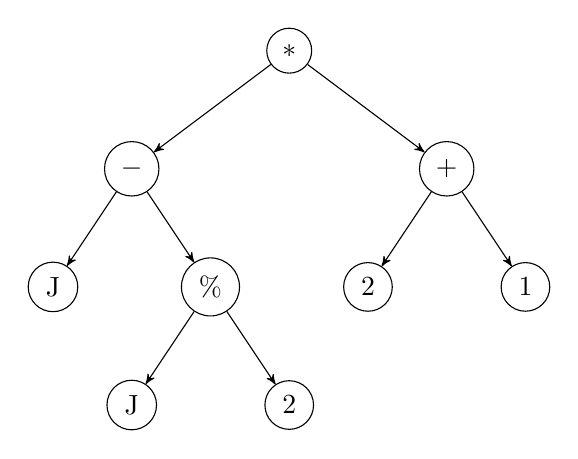
\begin{tikzpicture}[->,>=stealth',every node/.style={circle,draw},level 1/.style={sibling distance=4cm},level 2/.style={sibling distance=2cm}
]

\node[circle,draw](z){$*$}
 child{
    node[circle,draw]{$-$} child{node[circle,draw] {J}} child{node[circle,draw] {$\%$} child{node[circle,draw] {J}}  child{node[circle,draw] {2}}} }
  child{
    node[circle,draw]{$+$} child{node[circle,draw] {2}} child{node[circle,draw] {1}} };
\end{tikzpicture}}
\end{figure}
$\ \ *\ -\ J\ \%\ J\ 2\ +\ 2\ 1$

\end{column}
\end{columns}
\end{frame}

%------------------------------------------------
\begin{frame}
\frametitle{Fitness of a RNG}
\begin{itemize}
\item[-]The fitness of a RNG will be determined by the entropy of it's output.
\item[-]The entropy of a binary sequence is the evenness in the occurrence of a set of sub sequences in that sequence, and can be calculated using the formula below;
\begin{equation*}
E_{total} = \sum_{h = 1}^{N_{max}} \left[ - \sum_{j} P_{(hj)}\ \log_2\ P_{(hj)} \right]
\end{equation*}
\item[-]The fitness function in the GP will implement this equation to calculate he entropy and therefore fitness of each of the RNGs output. $N_{max}$ will be 7 in order to calculate the entropy for subsequence lengths from 1 to 7. 
\item[-]The maximum fitness a RNG can obtain is; 
\begin{equation*}
E_{max}=\sum_{i = 1}^{7} i =28
\end{equation*}
\end{itemize}
\end{frame}

%------------------------------------------------
\begin{frame}
\frametitle{Crossover}
Crossover will be the operator used to breed new RNG trees. It works by selecting$^{(1)}$ two parent trees with two random crossover points$^{(2)}$ which point to the root of a sub tree in each parent. These subtrees are swapped to create two new offspring trees.\\~\\
\begin{itemize}
\item[\ \ (1)]The two parents are selected using two different methods. Fitness Proportionate Reproduction gives members of the population with a higher fitness a greater probability of being selected. The second method is where one of the parents is selected relative to their fitness and the other uniformly.\\~\\
\item[\ \ (2)]The probability of choosing an internal (function) to an external (terminal) crossover point is user defined as an input parameter.\\~\\
After Crossover, the output and fitness of every individual in the population is recalculated.
\end{itemize}
\end{frame}

%------------------------------------------------
\begin{frame}
\frametitle{Outputs \& Termination}
After every generation, the data for that population is written to a file;
\begin{figure}[H]
\caption{Outputs}
\resizebox{10cm}{1.7cm}{
\begin{tabular}{l*{6}{l}r}
Data Type             & Output description\\
\hline
Integer & Generation number\\
Double & Generation run time in seconds \& hundredths of a second \\
Double & Total entropy/fitness of fittest candidate\\
Double & Entropy for subsequence size 1 of fittest candidate\\
\ \ \ \ $\vdots$ & \ \ \ \ \ \ \ \ \ \ \ \ \ \ \ \ \ \ \ \ \ \ \ \ $\vdots$\\
Double & Entropy for subsequence size 7 of fittest candidate\\
Boolean & Entropy of fittest candidate is $\geq$ target fitness?\\
String & Prefix expression for fittest candidate\\
\end{tabular}}\\~\\
\end{figure}
This data can be used for evaluation of the program.\\~\\
If the current generation count is equal to the user defined maximum, or the fitness of the fittest candidate is greater than or equal to the user defined target, the GP terminates. Otherwise process continues, until one of these criteria is met.
\end{frame}
%SNGP APPROACH
%------------------------------------------------
\subsection{Single Node Genetic Programming Design}
\begin{frame}
\frametitle{Single Node Genetic Programming Approach}
\begin{columns}[T]
\begin{column}{0.75\textwidth}
\begin{itemize}
\item[-]The aim is again to evolve a RNG, but in this case using the Single Node Genetic Programming (SNGP) methodology.
\item[-]There are fewer input parameters to the a SNGP  as shown in the figure below;
\begin{figure}
\caption{SNGP Input parameters}
\resizebox{7.6cm}{1.1cm}{
\begin{tabular}{l*{6}{l}r}
Data Type             & Input description\\
\hline
Integer & Length of a run (number of $smut$ operations)\\
Integer & Population size (number of nodes)\\
Double & Total (i.e. sum of) target fitness value\\
\end{tabular}}
\end{figure}

\end{itemize}
\end{column}
\begin{column}{0.35\textwidth}
\begin{figure}[H]
\caption{SNGP Flowchart}
\resizebox{3.5cm}{6.5cm}{
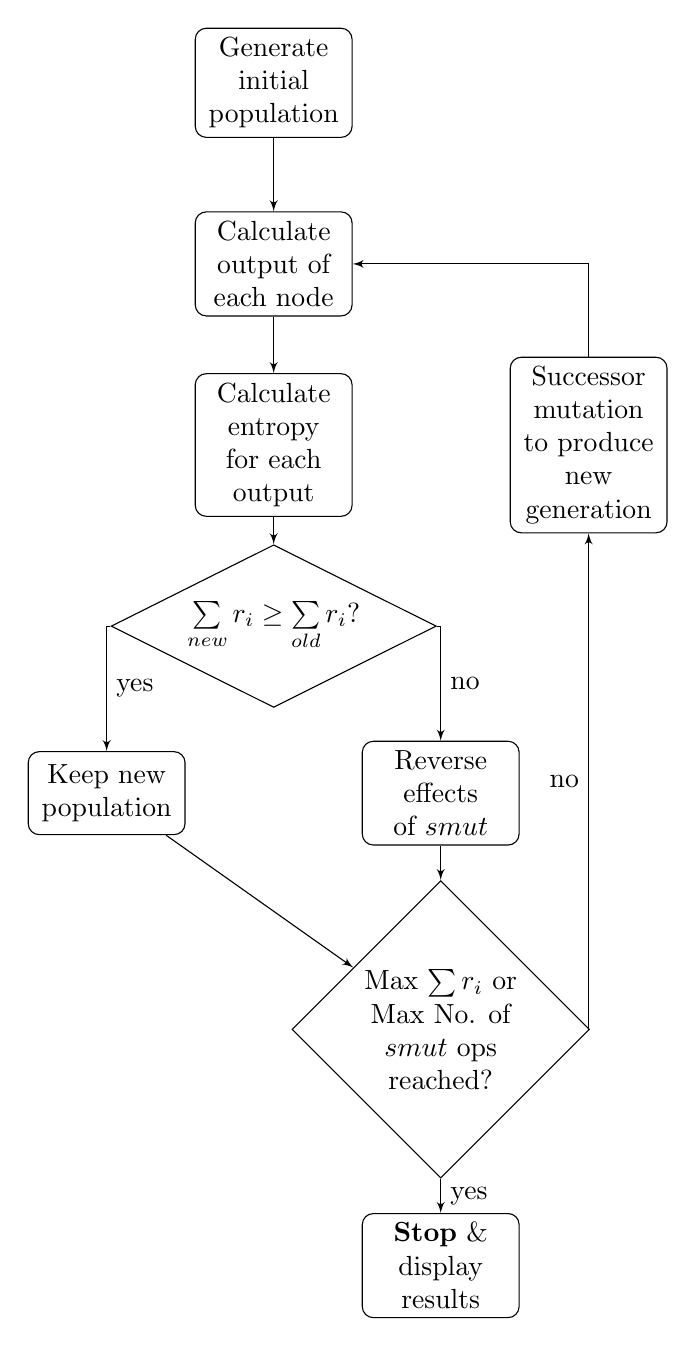
\begin{tikzpicture}[node distance = 2.3cm, auto]
    % Place nodes
    \node [block] (init) {Generate initial population};
    \node [block, below of=init] (identify) {Calculate output of each node};
    \node [block, below of=identify] (evaluate) {Calculate entropy for each output};
    \node [block, right of=evaluate, node distance=4cm] (update) {Successor mutation to produce new generation};
   
 \node [draw, diamond, aspect=2,  below of=evaluate] (decide1) {$\sum\limits_{new} r_i \geq \sum \limits_{old} r_i$?};
    \node [block, below left of=decide1, node distance=3cm] (greater) {Keep new population};
   \node [block, below right of=decide1, node distance=3cm] (less) {Reverse effects of $smut$};
    \node [decision, below of=less] (decide2) {Max $\sum r_i$ or Max No. of $smut$ ops reached?};
    
\node [block, below of=decide2, node distance=3cm] (stop) {\textbf{Stop} \& display results};
    % Draw edges
    \path [line] (init) -- (identify);
    \path [line] (identify) -- (evaluate);
    \path [line] (evaluate) -- (decide1);
    \path [line] (decide1) -| node  [near end]{yes} (greater);
    \path [line] (decide1) -| node [near end] {no} (less);
    \path [line] (less) -- (decide2);
    \path [line] (greater) -- (decide2);
    \path [line] (decide2) -| node [near end] {no} (update);
    \path [line] (update) |- (identify);
    \path [line] (decide2) -- node {yes}(stop);
\end{tikzpicture}}
\end{figure}
\end{column}
\end{columns}

\end{frame}

%------------------------------------------------
\begin{frame}
\frametitle{SNGP Structure}
\begin{itemize}
\item[-]A population is a set $M$ of $N$ tuples;
\begin{center}
$M = \{m_0,\ m_1,\ ...,\ m_{N-1}\}$ where; $m_i = \ <u_i,\ r_i,\ S_i,\ P_i,\ O_i>$ where;\\~\\
\end{center}
$u_i \in \{T \cup F\}$ - node in the terminal or function set\\
$r_i$ - fitness of the node\\
$S_i$ - set of successors of the node\\
$P_i$ - set of predecessors of the node\\
$O_i$ - output vector for this node\\~\\
\item[-]In C the population will be implemented as an array of N $structs$, where the $structs$ will represent the tuple above.
\item[-]The SNGP population represents a single graph structure.


\end{itemize}
\end{frame}

%------------------------------------------------
\begin{frame}
\frametitle{Graph Structure}
\begin{itemize}
\item[-]SNGP makes use of Dynamic Programming. When evaluating a tree the outputs of the successor nodes are used rather than calculating them from scratch. Giving it efficiency gains over conventional GP.\\~\\
\item[-]Every node in the graph is evaluated as the root node for a tree. Therefore there are as many RNG trees as there are nodes in the population, and these trees can be evaluated using the same method as the GP method.\\~\\
\item[-]The same fitness function is used to calculate the entropy of a RNG output. (Pseudocode for all main methods are available in the design document);\\
 \begin{center}$E_{total} = \sum_{h = 1}^{7} \left[ - \sum_{j} P_{(hj)}\ \log_2\ P_{(hj)} \right]$\end{center}


\end{itemize}
\end{frame}

%------------------------------------------------
\begin{frame}
\frametitle{Inital Generation}
The initial population (of the size defined by the user) is generated by adding all the elements in the terminal set exactly once, and then populating the rest with random nodes in the function set. The two successors for a function node are randomly selected from the existing population and added to $S_i$. $P_i$ is then updated in the successor nodes. The outputs and fitnesses are calculated as the nodes are being added.
\end{frame}

%------------------------------------------------
\begin{frame}
\frametitle{Successor Mutation}
SNGP makes use of one evolutionary operator, Successor Mutation or $smut$. This is where one element in $S_i$ in a node is randomly changed to another (deeper) node in the population.

\begin{figure}[H]
\caption{Successor Mutation}
\label{smutexample}
\resizebox{10cm}{3cm}{
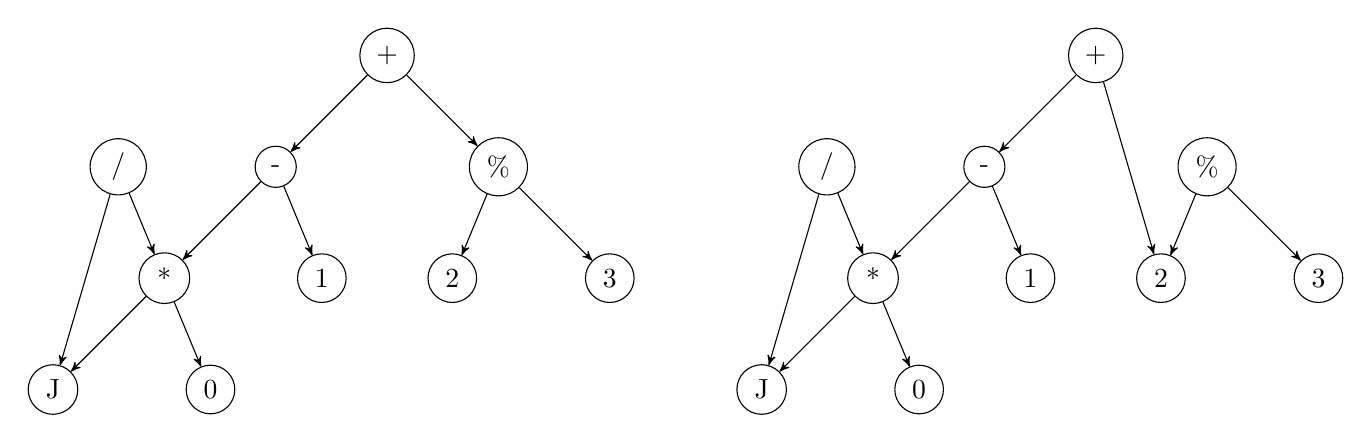
\begin{tikzpicture}[->,>=stealth',auto,node distance=2cm]

  \node[circle, draw] (+) {+};
  \node[circle, draw] (-) [below left of=+] {-};
  \node[circle, draw] (/) [left of=-] {/};
  \node[circle, draw] (*) [below left of=-] {*};
  \node[circle, draw] (mod) [below right of=+] {\%};
  \node[circle, draw] (J) [below left of=*] {J};
  \node[circle, draw] (0) [right of=J] {0};
  \node[circle, draw] (1) [right of=*] {1};
  \node[circle, draw] (3) [below right of=mod] {3};
  \node[circle, draw] (2) [left of=3] {2};

  \path[every node/.style={font=\sffamily\small}]
    (+) edge node [left] {} (-)
	 edge node [right] {} (mod)
        
    (-) edge node [right] {} (1)
	edge node [left] {} (*)
        
    (/) edge node [right] {} (*)
         edge node [left] {} (J)

    (*) edge node [left] {} (J) 
	edge node [right] {} (0)
        
    (mod) edge node [right] {} (3)
		edge node [left] {} (2);

\begin{scope}[xshift=9cm]
  \node[circle, draw] (+) {+};
  \node[circle, draw] (-) [below left of=+] {-};
  \node[circle, draw] (*) [below left of=-] {*};
  \node[circle, draw] (/) [left of=-] {/};
  \node[circle, draw] (mod) [below right of=+] {\%};
  \node[circle, draw] (J) [below left of=*] {J};
  \node[circle, draw] (0) [right of=J] {0};
  \node[circle, draw] (1) [right of=*] {1};
  \node[circle, draw] (3) [below right of=mod] {3};
  \node[circle, draw] (2) [left of=3] {2};

  \path[every node/.style={font=\sffamily\small}]
    (+) edge node [left] {} (-)
	 edge node [right] {} (2)
        
    (-) edge node [right] {} (1)
	edge node [left] {} (*)
        
    (/) edge node [right] {} (*)
         edge node [left] {} (J)

    (*) edge node [left] {} (J) 
	edge node [right] {} (0)
        
    (mod) edge node [right] {} (3)
		edge node [left] {} (2);
\end{scope}
\end{tikzpicture}}

\begin{center}
Before:
$\{J\}$, 
$\{0\}$, 
$\{1\}$, 
$\{2\}$, 
$\{3\}$, 
$\{* \ J \ 0\}$,
$\{/ \ J\ *\ J\ 0\}$, 
$\{-\ *\ J \ 0 \ 1\}$, 
$\{\%\ 2\ 3\}$,
$\{+\ -\ *\ J \ 0 \ 1 \ \%\ 2 \ 3\}$.
\end{center}
\begin{center}After: $\{J\}$, $\{0\}$, $\{1\}$, $\{2\}$, $\{3\}$, $\{* \ J \ 0\}$, $\{/ \ J\ *\ J\ 0\}$, $\{-\ *\ J \ 0 \ 1\}$, $\{\%\ 2\ 3\}$, $\{+\ -\ *\ J \ 0 \ 1 \ 2\}$\end{center}

\end{figure}
\end{frame}

%------------------------------------------------

\begin{frame}
\frametitle{Outputs and Termination}
The outputs for SNGP are the exact same as those for GP. This will make comparing and evaluating both approaches simpler.\\~\\
If the current generation count is equal to the user defined maximum, or the sum of all the fitness values for all nodes ($\sum r_i$) is greater than or equal to the user defined target, the program terminates. Otherwise process continues, until one of these criteria is met.
\end{frame}


%EVALUATION DESIGN
%------------------------------------------------
\subsection{Evaluation Design}
\begin{frame}
\frametitle{Evaluation Design}
GP vs SNGP. To compare GP and SNGP, we must form test cases for matching inputs of both methodologies. There are three matching inputs as shown in the figure below, and the other inputs will remain as constant for all test cases as in the figure below that.


\begin{figure}[H]
\centering
\caption{Matching parameters}
\label{inputforboth}
\resizebox{8cm}{0.7cm}{
\begin{tabular}{l*{6}{l}r}
Data Type             & Input description\\
\hline
Integer & Maximum number of generations / Length of a run (number of $smut$ operations)\\
Integer & Population size; number of trees (GP) or number of nodes (SNGP)\\
Double & Target fitness value (GP), Target fitness value for sum of all node targets (SNGP) \\
\end{tabular}}
\end{figure}

\begin{figure}[H]
\centering
\caption{Remaining constant parameters for GP}
\label{loparam}
\resizebox{7cm}{1cm}{
\begin{tabular}{l*{6}{l}r}
Data Type             & Input description & Values\\
\hline
Integer & Maximum initial program depth & 4\\
Integer & Maximum crossover program depth & 15\\
Double & Fitness proportionate reproduction probability & 0.1\\
Double & Crossover operation probability & 0.9\\
Double & Internal node crossover probability & 0.9\\
Double & External node crossover probability & 0.1\\
\end{tabular}}
\end{figure}

\end{frame}

\newcommand\scalemath[2]{\scalebox{#1}{\mbox{\ensuremath{\displaystyle #2}}}}
%------------------------------------------------
\begin{frame}
\frametitle{Test Cases}
I formed 8 test cases, two different values for each of the three inputs over all combinations;

\footnotesize
\arraycolsep=3pt % default: 5pt
\medmuskip = 1mu % default: 4mu plus 2mu minus 4mu
\[ \bordermatrix{~ &  1&  2& 3& 4& 5 & 6 & 7 & 8\cr
                  $Max Gen/$smut& 51 & 51 & 101 & 101& 101 & 101 & 51 & 51   \cr
                  $Pop size$& 500 & 1000 & 500 & 1000 & 500 & 1000 & 500 & 1000  \cr
	       $Targ Fit$ & 27.990 & 28.0 & 27.990 & 28.0 & 28.0 & 27.990 & 28.0 & 27.990 \cr}
\]

\end{frame}


%------------------------------------------------
\begin{frame}
\frametitle{Test Criteria}
Test criteria for GP vs SNGP
\begin{itemize}
  \item[1)]
  Average entropy fitness of fittest member over 100 runs
  \item[2)]
  Average solution rate over 100 runs
  \item[3)]
 Average minimum and maximum solution size over 100 runs
  \item[3)]
Average run time over 100 runs
  \item[4)]
Generation run time over one run
  \item[5)]
Average solution size over one run
  \item[6)]
Entropy climb over one run
  \item[7)]
 Scalar entropies over one run
\end{itemize}
\end{frame}

%------------------------------------------------
\begin{frame}
\frametitle{Other Random Number Generators}
\begin{itemize}
\item[-]Test the fittest RNGs produced by GP and SNGP against the Pseudo Random Number Generator in the C programming language. Using the same entropy calculation in the fitness function.\\~\\
\item[-]Test the fittest RNGs produced by GP and SNGP against the True Random Number Generator at \emph{www.random.org}, where up to 1,000,000 randomly generated bits can be sent in HTTP packets from a piece of hardware that measures atmospheric noise. From  this bit sequence we can measure it's entropy and therefore compare results.
\end{itemize}
\end{frame}

%------------------------------------------------
\section{Plan Progress}
\begin{frame}
\frametitle{Plan Progress}


\begin{figure}

\resizebox{11.5cm}{6cm}{
\centering
\begin{ganttchart}[y unit title=0.4cm,
y unit chart=0.5cm,
vgrid,hgrid, 
title label anchor/.style={below=-1.6ex},
title height=1,
bar/.style={fill=gray!50},
bar/.append style={fill=gray!100},
bar incomplete/.append style={fill=gray!50},
incomplete/.style={fill=white},
progress = today,
today = 10, 
bar height=0.7,
group right shift=0,
group top shift=.6,
group height=.3,
group peaks height =.2,
milestone/.append style={fill=gray!50}
]
{1}{34}
%labels
\gantttitle{Final Year Project}{34} \\
\gantttitle{Sep}{2} 
\gantttitle{Oct}{4} 
\gantttitle{Nov}{4} 
\gantttitle{Dec}{4} 
\gantttitle{Jan}{4} 
\gantttitle{Feb}{4} 
\gantttitle{Mar}{4} 
\gantttitle{Apr}{4} 
\gantttitle{May}{4} \\
%tasks
\ganttbar{Research}{1}{6} \\
\ganttgroup{Specification}{2}{4} \\
\ganttbar{Write Specification}{2}{4} \\
\ganttgroup{Design}{5}{10} \\
\ganttbar{Plan Design}{5}{5}\\
\ganttbar{Write Design Document}{6}{9}\\
\ganttbar{Plan Presentation}{9}{9}\\
\ganttbar{Give Design Presentation}{10}{10} \\
\ganttmilestone{Implementation Documentation Complete}{10}\\
\ganttgroup{Implementation}{11}{26} \\
\ganttbar{Implement Koza's PRNG GP}{11}{18}\\
\ganttbar{Implement SNGP Approach}{19}{23} \\
\ganttbar{Compare GP vs SNGP}{24}{26}\\
\ganttmilestone{Implementation Complete}{26} \\
\ganttgroup{Demonstration}{27}{28} \\
\ganttbar{Write/Plan Demonstration}{27}{27} \\
\ganttbar{Give Demonstration}{28}{28} \\
\ganttgroup{Dissertation}{29}{34} \\
\ganttbar{Plan Dissertation}{29}{29}\\
\ganttbar{Write Dissertation}{30}{34} \\
\ganttmilestone{Project Completed}{34} \\

%relations
\ganttlink[link type=dr]{elem2}{elem4} 
\ganttlink[link type=dr]{elem4}{elem5}
\ganttlink[link type=dr]{elem4}{elem6}
\ganttlink[link type=dr]{elem5}{elem8}
\ganttlink[link type=dr]{elem6}{elem7}
\ganttlink[link type=dr]{elem7}{elem8} 
\ganttlink[link type=dr]{elem8}{elem10} 
\ganttlink[link type=dr]{elem10}{elem11}
\ganttlink[link type=dr]{elem10}{elem12}
\ganttlink[link type=dr]{elem11}{elem12}
\ganttlink[link type=dr]{elem12}{elem13} 
\ganttlink[link type=dr]{elem13}{elem15}
\ganttlink[link type=dr]{elem15}{elem16}
\ganttlink[link type=dr]{elem16}{elem18}
\ganttlink[link type=dr]{elem18}{elem19}
\ganttlink[link type=dr]{elem19}{elem20}

\end{ganttchart}}
\caption{Gantt Chart - Work plan}
\label{fig:ganttchart}
\end{figure}

\end{frame}



\begin{thebibliography}{2}
\bibitem{kozarng}
  John R. Koza, 
  \emph{Evolving a Computer Program to Generate Random Numbers Using the Genetic Programming Paradigm}. 
  Stanford University, 
  1991.

\bibitem{jacksonsngp2}
  David Jackson,
  \emph{A New, Node-Focused Model for Genetic Programming}.
  Proceedings of the 15th European Conference on Genetic Programming, EuroGP 2012, 
  Springer Verlag
  2012.
\end{thebibliography}

\begin{frame}
\begin{center}Q\&A\end{center}
\end{frame}
\end{document} 